\chapter{\IfLanguageName{dutch}{Opsplitsen en herstructureren van de backend}{Splitting up and restructuring the backend}}
\label{ch:opsplitsen-backend}

In de volgende fase van het onderzoek was het herstructureren van de backend en het opdelen in drie afzonderlijke services, de cruciale eerste stap in de omschakeling van monoliet naar services. 
\begin{figure}
	\centering	
	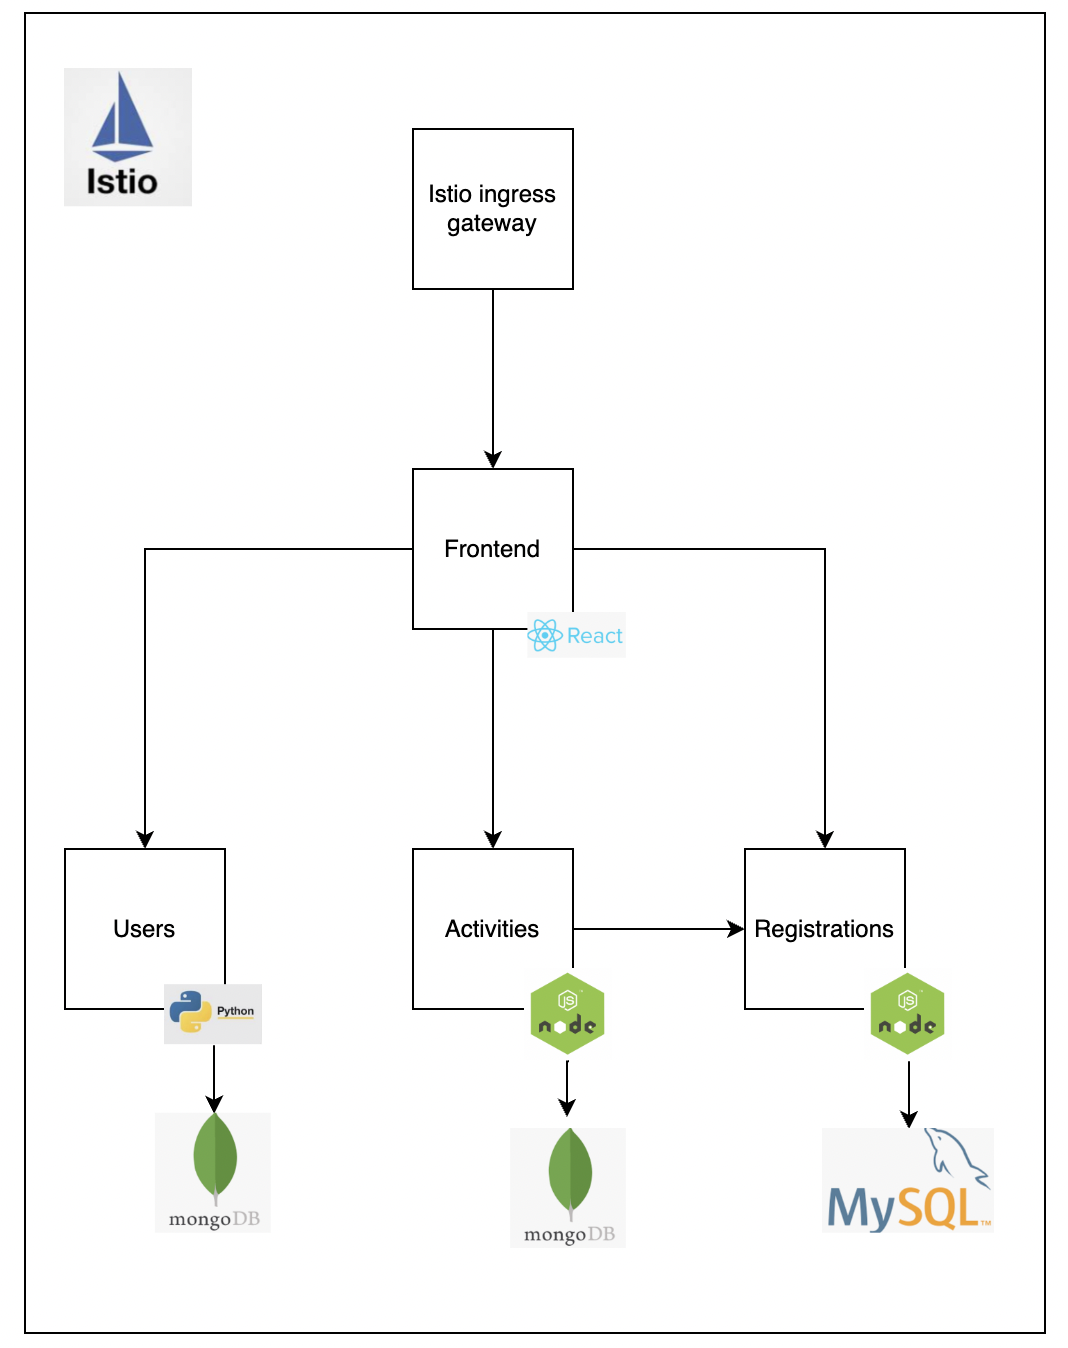
\includegraphics[width = 8cm]{services.png} 
	\caption{Architectuur services} 
	\label{fig:services} 
\end{figure}
\FloatBarrier

Er zijn drie services gedefinieerd: een gebruikersservice, een activiteitenservice en een registratieservice. Deze services zijn verantwoordelijk voor respectievelijk het beheren van gebruikersgegevens, activiteiten en registratiegegevens. Door deze services te scheiden, kan elke service onafhankelijk worden ontwikkeld, getest en geschaald.

Voor gebruikers- en activiteitengedeelte werd gekozen om gebruik te maken van een NoSQL-database, omdat deze data statisch is en niet vaak verandert. Voor het registratiegedeelte werd gekozen voor een relationele database, omdat deze data vaak verandert en er veel transacties zijn.

Allereerst werd het gebruikersgedeelte getransformeerd van Node.js naar Python, waarbij ervoor gezorgd werd dat het zijn gegevens ophaalde uit een MongoDB-database.

Het omzetten van de data van MySql naar MonogDB is gebeurd door de data te exporteren naar een JSON-bestand en vervolgens te importeren in de MongoDB-database.

Het activiteitengedeelte van de backend heb ik echter in Node.js gehouden, waarbij ervoor gezorgd is dat het ook zijn gegevens ophaalt uit de MongoDB-database.

Het registratiegedeelte van de backend blijft ook in Node.js, maar blijft gebruik maken van een MySQL-database voor gegevensopslag. Deze keuze is gebaseerd op de specifieke vereisten van het registratieproces, waarbij MySQL wordt gekozen vanwege zijn robuuste transactiemogelijkheden en uitstekende ondersteuning voor relationele gegevensmodellering. Het gebruik van een aparte databaseoplossing voor dit gedeelte van de backend stelt me in staat om optimaal te profiteren van de unieke kenmerken en voordelen van MySQL. De code moet worden aangepast omdat gebruikers en activiteiten nu aparte services zijn. Deze moeten worden aangeroepen vanuit de registratieservice. Om onafhankelijk van deze services te kunnen ontwikkelen, worden deze in eerste instantie vervangen door stubs.

Technisch gezien wordt de Python-code van de backend uitgevoerd in Unicorn, een lightweight ASGI (Asynchronous Server Gateway Interface) compatibele webserver voor Python. Een `service.py`-bestand wordt gebruikt om de service te starten en alle endpoints te definiëren. De keuze voor Unicorn als ASGI-server biedt een robuuste en betrouwbare uitvoeringsomgeving voor Python-toepassingen. Door de ondersteuning voor asynchrone verwerking van aanvragen kunnen optimale prestaties en schaalbaarheid worden gegarandeerd.

Aan de andere kant wordt het Node.js-gedeelte van de backend uitgevoerd met behulp van Express, waarbij een `express.js`-bestand wordt gebruikt om de service te starten en alle endpoints te definiëren. Express staat bekend om zijn eenvoud en flexibiliteit, waardoor het een populaire keuze is voor het ontwikkelen van webapplicaties in Node.js. Door gebruik te maken van Express kan ik snel en efficiënt RESTful API's implementeren en beheren.

Het feit dat deze services lokaal op verschillende poorten draaien, draagt bij aan de isolatie en modulariteit van het systeem, waardoor elk onderdeel onafhankelijk kan worden ontwikkeld, getest en geschaald. Deze aanpak is de eerste stap in het omzetten van de monoliet naar een microservice.

In figuur \ref{fig:getUserLocal} is te zien hoe de gebruikersgegevens worden opgehaald uit de MongoDB-database lokaal op poort 9080.

\begin{figure}
	\centering	
	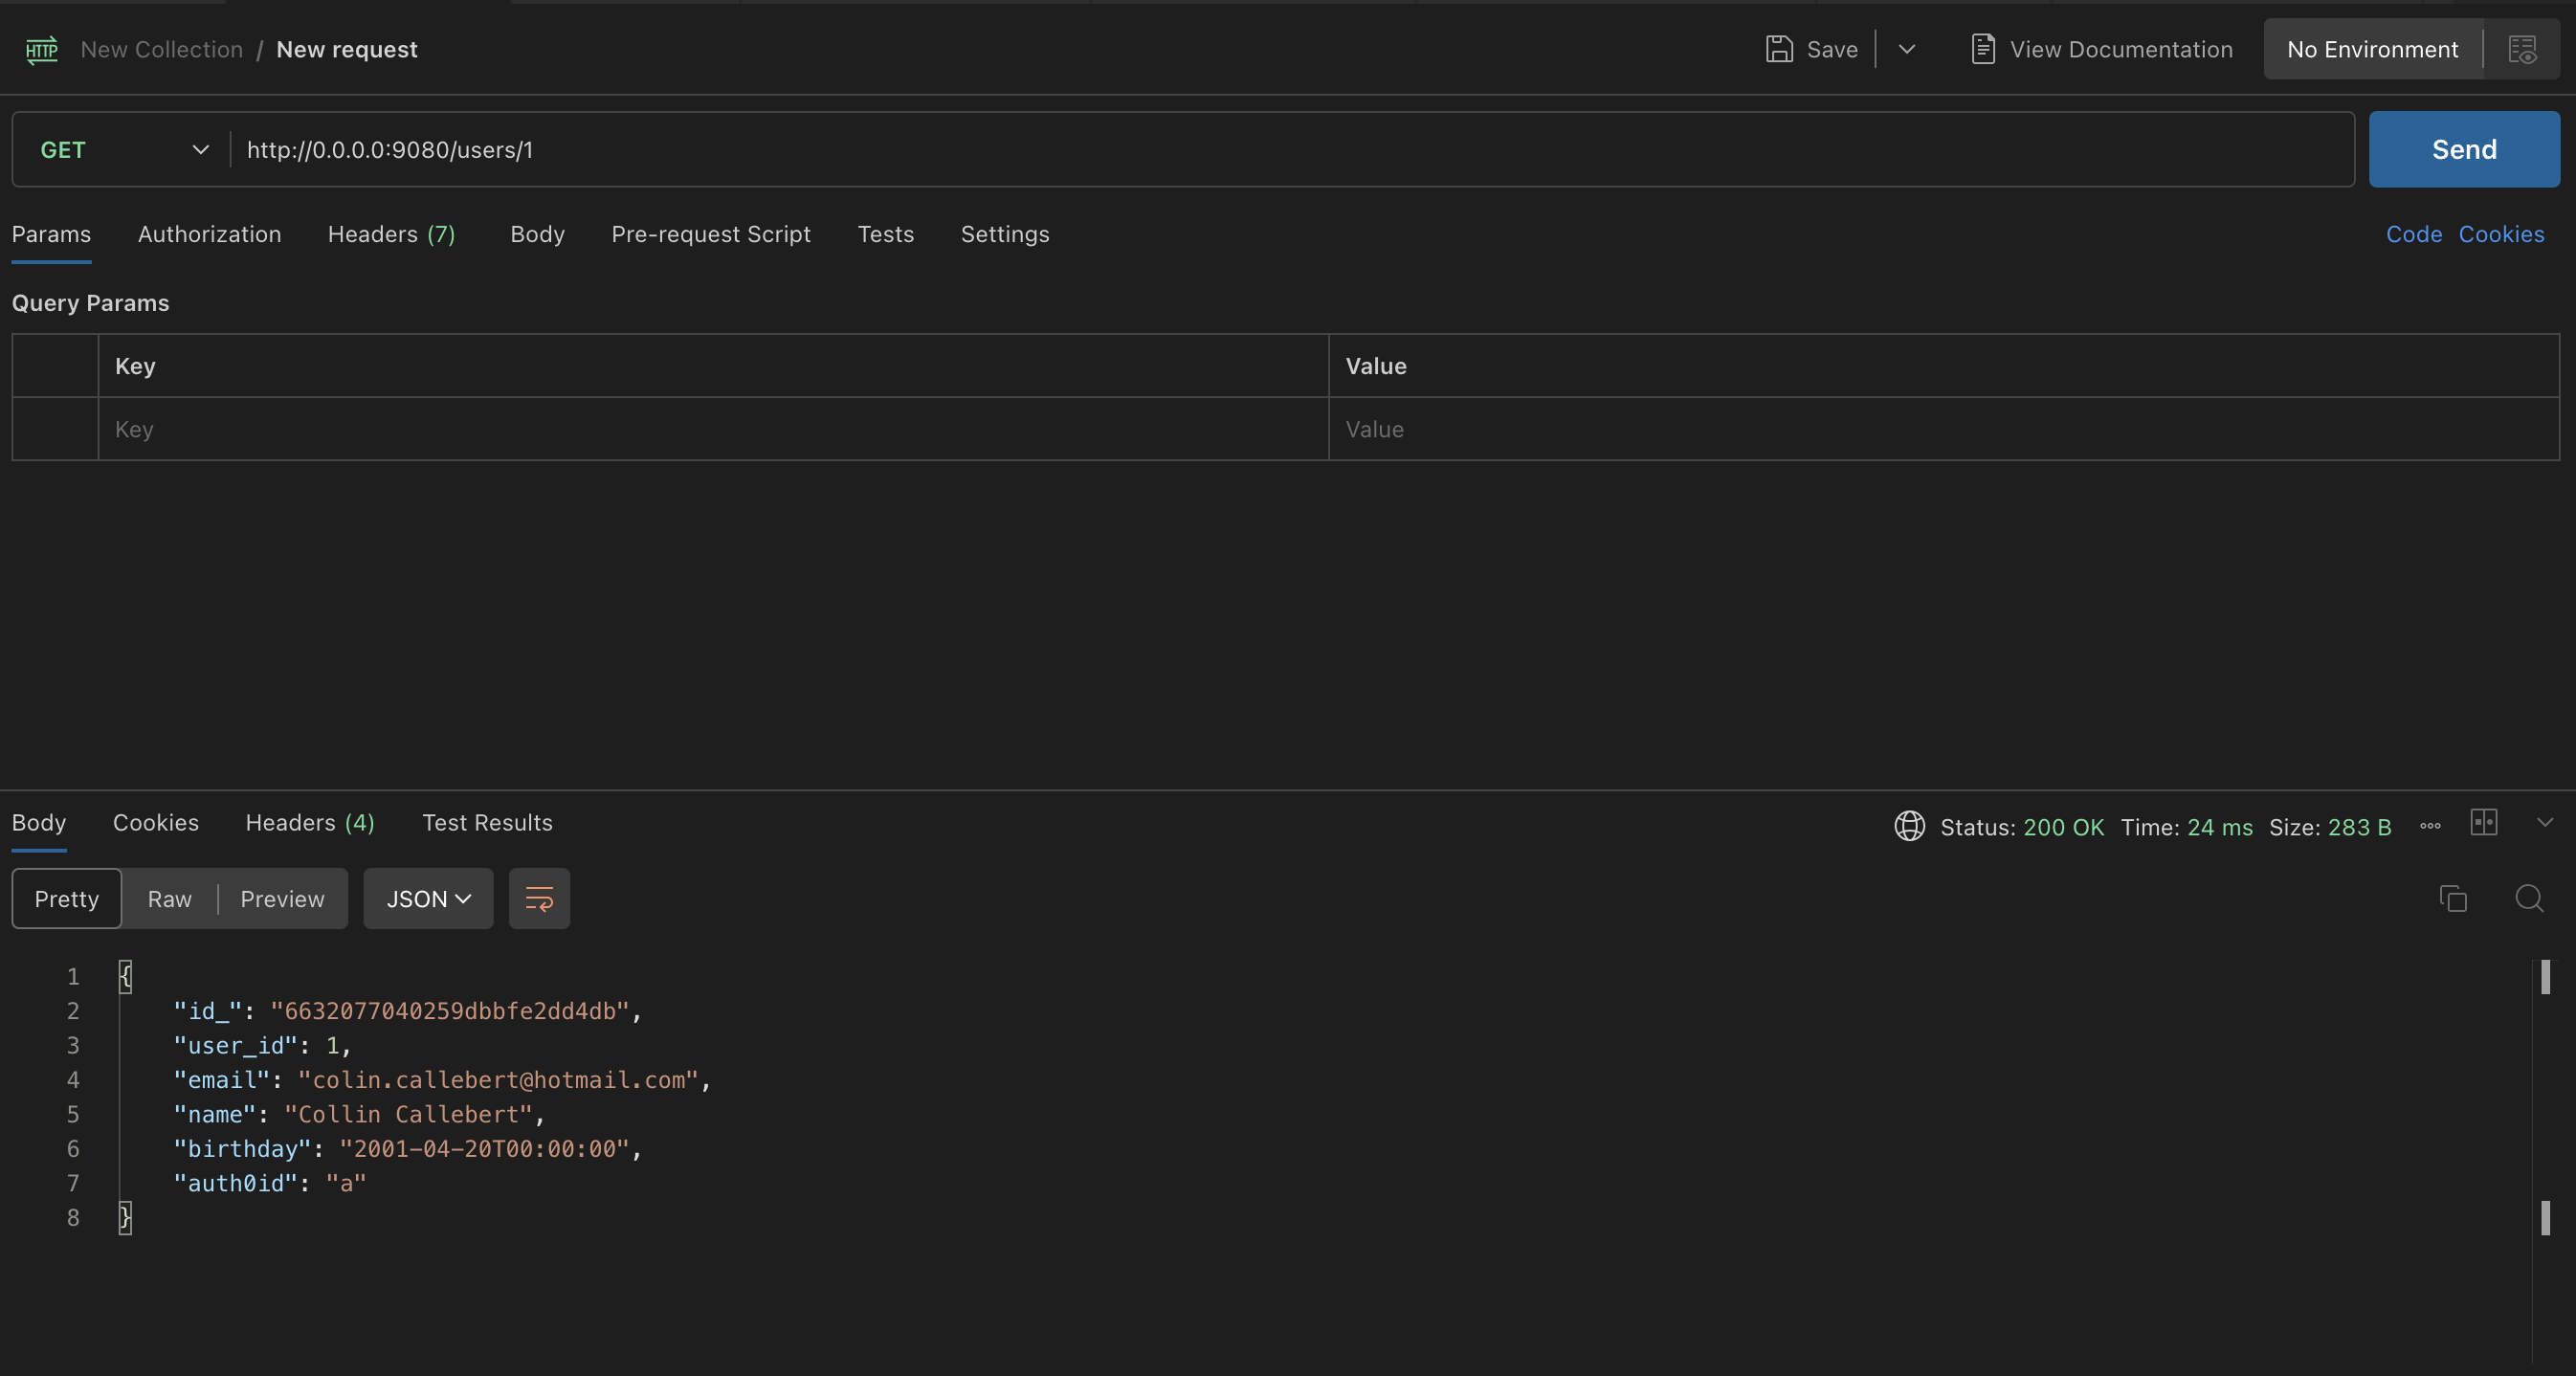
\includegraphics[width = 16cm]{getUserLocal.png} 
	\caption{Haal gebruikersgegevens op uit de MongoDB-database lokaal}
	\label{fig:getUserLocal} 
\end{figure}
\FloatBarrier